\section{Introduction}
\label{sec:introduction}

% state the learning objective 
The objective of this laboratory assignment is to compare the mesh method and nodal method to the values of current and voltage of the simulated circuit and see how accurate they are. The circuit can be seen in Figure ~\ref{fig:rc}. 

\begin{figure}[h] \centering
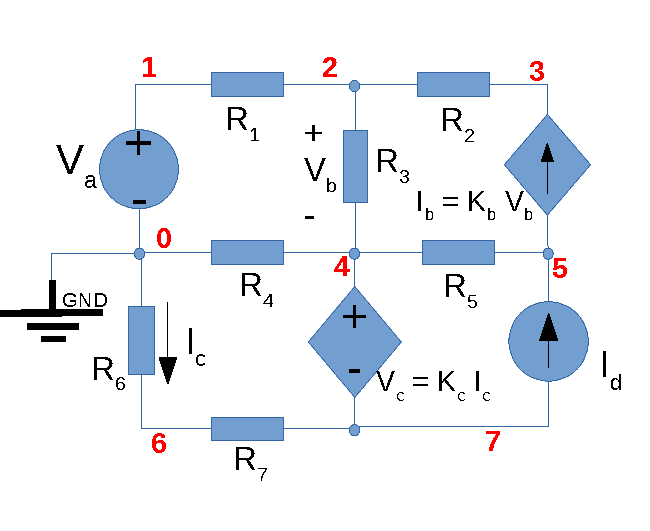
\includegraphics[width=0.6\linewidth]{rcm.pdf}
\caption{Nodal representation of the circuit.}
\label{fig:rc}
\end{figure}


In section 2, a theoretical analysis of the circuit is presented. In section 5, the circuit is analyzed by simulation, and the results are compared to the theoretical results obtained in section 2. Finally, in section 6, we conclude our study.


